% JAC v4 (2026-09-12) — release v2.0.0. Zenodo DOI: 10.5281/zenodo.22725070 (https://doi.org/10.5281/zenodo.22725070). Source repository: https://github.com/Nyx-Dynamics/doxypep-bystander
% JAC Supplementary data — standalone, compiles independently of the main article.
% TEMPLATE_PENDING: portable LaTeX; migrate into official JAC/OUP supplement
% format when supplied. All material here is RELOCATED from the validated
% manuscript/repository, not newly generated. Every item is cited in the main
% article (Materials and methods and Results). Full per-document coding tables,
% the frozen literature-search snapshot, and all analysis outputs regenerate from
% the public repository (make all; outputs/) and are archived at the cited DOI.
\documentclass[11pt,a4paper]{article}
\usepackage[T1]{fontenc}
\usepackage[utf8]{inputenc}
\usepackage{lmodern}
\usepackage{amsmath,amssymb}
\usepackage{textcomp}
\usepackage{graphicx}
\usepackage{booktabs}
\usepackage{tabularx}
\usepackage[margin=1in]{geometry}
\usepackage{caption}
\usepackage{url}\urlstyle{tt}
\usepackage{parskip}
\graphicspath{{figures/}}

\newcommand{\sa}{\emph{S.~aureus}}
\newcommand{\Sa}{\emph{Staphylococcus aureus}}

\title{\textbf{Supplementary data}\\[6pt]
\large Guidance and surveillance capability for bystander \Sa{} tetracycline
resistance under doxy-PEP: a three-stream evidence audit}
\author{Adrian C. Demidont}
\date{}

\begin{document}
\maketitle
\thispagestyle{empty}

\noindent All supplementary material is relocated from the validated analysis and
regenerates from the public repository (\texttt{make all}; \texttt{outputs/}),
archived with a citable DOI. \textit{JAC} nomenclature conventions are followed
and MICs are expressed in mg/L.

% ===================================================================
\section*{S1. The measurement-inheritance schema}

We make the construct operational so it can be applied beyond this case. Treat the
answerability of a question as requiring a measurement vector
\[M=\{\,U,\ E,\ P,\ D,\ T,\ L,\ R\,\}\]
where $U$ is the unit/population, $E$ the exposure, $P$ the phenotype/outcome, $D$
the denominator, $T$ the temporal structure/cadence, $L$ the linkage at which $E$
and $P$ are joined, and $R$ the locus of measurement responsibility. Measurement
inheritance occurs when a downstream system retains the dimensions appropriate to
the upstream question but not those the downstream estimand requires. A
distributive corollary follows when the benefit and the potential downstream harm
accrue to different populations ($B\neq H$): the beneficiary population $B$ remains
represented by the inherited $\{U,E,P,D,L\}$, while the population $H$ that would
bear an externalised consequence is represented by none of them jointly. The three
streams instantiate the schema directly (Table~\ref{tab:vector}).

\begin{table}[h]
\centering
\caption{The measurement vector across the evidence chain. ``Present'' = the
dimension exists at the resolution the downstream question needs; ``wrong
unit/resolution'' = present but inherited from the upstream question; ``absent''
= not captured.}
\label{tab:vector}
\small
\begin{tabularx}{\textwidth}{@{}lXXX@{}}
\toprule
Dimension & Stream A (trial) & Stream B (guidance) & Stream C (surveillance)\\
\midrule
$U$ unit & Participant \sa{} & Not specified for \sa{} & MRSA subset (wrong unit)\\
$E$ exposure & Randomised doxy-PEP & Prescribing context & PrEP proxy only\\
$P$ phenotype & Incident doxy-R (present) & Not measured (absent) & Methicillin axis (wrong unit)\\
$D$ denominator & Randomised participants & None for \sa{} & Population, but methicillin\\
$T$ cadence & Time-to-event & None & Cross-sectional/facility\\
$L$ linkage & Individual & None assigned & No common $E$--$P$ denominator (absent)\\
$R$ responsibility & Trial investigators & Unassigned (absent) & Unassigned for tetracycline \sa{}\\
\bottomrule
\end{tabularx}
\end{table}

The two load-bearing gaps are $R$ in Stream B (no party assigned to measure the
bystander) and $L$ in Stream C (no deployed system joins doxy-PEP exposure to the
\sa{} tetracycline phenotype at a common denominator).

% ===================================================================
\section*{S2. Stream A --- supplementary trial analyses}

These analyses establish that the cross-sectional carriage endpoint could not
resolve the downstream population question under the observed designs and sampling
structure. They are MRSA-scoped (MRSA being a subset, not the analytic unit) and
are \emph{not} load-bearing for the individual-level result the final trial
resolved.

\begin{itemize}
\item \textbf{Detectability (interim).} For each first-party primary-trial \sa{}
arm comparison, exact-Fisher power and the minimum detectable RR at 80\% power
were computed from arm sizes and control rate against the external benchmark. None
of four comparisons was powered; the minimum detectable RR was 3.8--5.1 against a
benchmark of 1.42--2.25 (\path{outputs/detectability_result.md}).
\item \textbf{Duration/accrual.} Preserving each comparison's arm ratio and
control rate, the sample reaching 80\% power lands in the hundreds to thousands per
arm; the realised denominator reflects the early efficacy stop
(\path{outputs/duration_result.md}). No duration counterfactual is inferred from
the two arm-split visits.
\item \textbf{Clustering dispersion.} Between-cohort dispersion of MRSA
colonisation across independent MSM cohorts was estimated by a logit-normal
binomial random-effects model (Gauss--Hermite quadrature) as a conservative
external heterogeneity anchor (\path{outputs/dejong_sigma_result.md}).
\item \textbf{Trend-test degradation.} At the trials' per-visit denominators, a
naive cross-sectional trend test (Cochran--Armitage) is badly oversized under the
estimated dispersion, scoring a flat process as a significant trend most of the
time (\path{outputs/coverage_null_result.md}).
\item \textbf{Outbreak-shape non-identifiability.} Flat, monotone-trend and
outbreak-wave models fitted to the MRSA carriage series by maximum likelihood are
not distinguishable by AIC or parametric-bootstrap likelihood-ratio tests
(\path{outputs/three_outbreak_fit_result.md}).
\item \textbf{Mechanism-blind measurement in \sa{} (now in the main text).} In a
military antimalarial--doxycycline cohort of 168 personnel, overall
tetracycline-class resistance in \emph{S. aureus} did not differ by doxycycline
exposure while \emph{tet}(M) genes were significantly more common among the
exposed (p=0.031) --- a single breakpoint concealing a mechanism shift. This
cohort is \emph{S. aureus}-specific (not cross-organism); it is promoted to the
main-text phenotype-unit argument (Mende \textit{et al.}, \textit{Diagn Microbiol
Infect Dis} 2016;86:211--220).
\end{itemize}

The one positive within-arm trend statistic in this material is a published-figure
re-analysis of DOXYVAC MRSA carriage (1.8\% to 9.9\%), cited as such and not
originated here.

% ===================================================================
\section*{S3. Stream B --- guidance corpus and coding}

\textbf{Denominator.} The purposive denominator is the US jurisdictions with
documented community-associated MRSA/USA300 transmission in men who have sex with
men, defined by de Jong's systematic review and the outbreak literature it cites
--- the same source supplying the Stream A clustering dispersion. Governmental
public-health guidance only was assessed; clinic and provider-organisation
documents were excluded because they carry neither surveillance authority nor
monitoring policy.

\textbf{Coding.} Each document was coded from full text (not search snippets), one
record per document, every finding carrying a locator, for: whether it mandates
in-category monitoring (gonorrhoea, chlamydia, syphilis) and host-toxicity labs;
and whether it names, counsels on, or measures \sa{}. Bystander treatment was
graded silent / generic-microbiome / organism-named; \sa{} monitoring as required
/ suggested / silent / explicitly-none (the last requiring a verbatim quote).
Coding was blind to the expected outcome. The author identified, retrieved and
screened all source documents for eligibility from full text before any coding
pass; a first LLM pass coded all 10 documents against the prespecified schema, and
a second, blinded LLM pass (a chat interface rather than the command-line agent,
same model family) independently re-coded a 5-document subsample (25 field-codings,
chosen to span all \sa{}-location categories), with disagreements resolved by the
author against the source. Per-field agreement is reported as raw concordance:
92\% (23/25), and the single field with meaningful disagreement (bystander
treatment; $\kappa=0.58$, context only) is reported unrounded. Because the two
passes share a model family their errors are not independent (main-text
Limitations).

\textbf{Result.} Of the six documented-outbreak jurisdictions --- San Francisco,
Chicago, New York City, Boston (Massachusetts), Los Angeles County and San Diego
--- 0 require or suggest \sa{} monitoring; three name \sa{}, two invoke only a
generic microbiome risk, one is silent. An independence check from document
content (structure, shared passages, stated derivation) finds four independently
authored declines, with Los Angeles County adapted from San Francisco and
Massachusetts from an external template. Across the full coded corpus (10
documents: CDC, WHO and eight US jurisdictions) 0 instrument the bystander; a
further jurisdiction deferring to CDC inherits CDC's non-monitoring and is counted
separately. The full per-document coding table with locators is in the repository
(\texttt{data/processed/}).

% ===================================================================
\section*{S4. Stream C --- surveillance enumeration and dilution model}

\textbf{Enumeration.} A prespecified set of 12 established US surveillance and
data systems (federal, state or metropolitan) plausibly capable of capturing, at
the required level, either doxy-PEP/doxycycline exposure or \sa{} AMR phenotype was
coded on three capabilities: exposure capture, phenotype capture (of the \sa{}
tetracycline unit, not the MRSA subset) and the join. Two capture exposure at a
population denominator (AIDSVu; CDC AtlasPlus) as a PrEP proxy; zero capture \sa{}
tetracycline resistance at a population denominator. The population-based \sa{}
platform (ABCs/EIP) and the National Healthcare Safety Network report the
methicillin axis; the facility cumulative antibiogram is the only routine
tetracycline reading and carries no population denominator (CLSI M39 mandates the
MRSA/MSSA split and makes tetracycline a selectively suppressible supplemental
agent); the National Antimicrobial Resistance Monitoring System excludes \sa{}.
Tetracycline-resistant \sa{} is nationally notifiable nowhere. Surveillance
capability was assessed as of August 2026; Stream C was coded by a single pass
(unlike the double-coded Stream B), an asymmetry noted in the main-text
Limitations. The full inclusion/exclusion list with a reason per system is in
Table~\ref{tab:streamc}.

\begin{table}[h]
\centering
\caption{Stream C enumeration: 12 included US surveillance and data systems and
three excluded, each with a stated reason. No included system captures both
doxy-PEP exposure and the \sa{} tetracycline phenotype at a common population
denominator (0/12 join).}
\label{tab:streamc}
\small
\begin{tabularx}{\textwidth}{@{}p{0.30\textwidth}>{\raggedright\arraybackslash}X@{}}
\toprule
System & Capability / reason\\
\midrule
\multicolumn{2}{@{}l}{\emph{Included (12)}}\\
AIDSVu & Exposure only, PrEP proxy at population denominator; no phenotype\\
CDC NCHHSTP AtlasPlus & Exposure only, PrEP proxy at population denominator; no phenotype\\
NHSN Antimicrobial Use Option & Inpatient antimicrobial use, no population denominator; not doxy-PEP\\
State PDMPs & Do not capture doxy-PEP dispensing as such; no phenotype\\
Metro STD/HIV sentinel surveillance & Sentinel exposure, no population denominator; no \sa{} phenotype\\
NARMS & Excludes \sa{} altogether\\
GISP / eGISP & Gonococcal isolates only (wrong organism)\\
ABCs / EIP invasive \sa{} & Population-based, but methicillin (MRSA/invasive) --- wrong phenotype unit\\
NHSN AR Option / MRSA LabID & MRSA events; facility, no population denominator\\
AR Lab Network (ARLN) & Isolate referral; no exposure link, no population denominator\\
NNDSS & Tetracycline-resistant \sa{} is not notifiable\\
Hospital cumulative antibiograms & Only routine tetracycline reading, but non-standardised and no population denominator\\
\addlinespace
\multicolumn{2}{@{}l}{\emph{Excluded (3)}}\\
CDC Find Doxy PEP directory & A provider/location directory, not surveillance\\
Commercial AST networks (ATLAS, BD, PINC AI, IQVIA) & Commercial convenience datasets; no population denominator\\
Doxy-PEP RCTs and cohorts (DoxyPEP, DOXYVAC, Soge) & One-off research studies, not deployed surveillance\\
\bottomrule
\end{tabularx}
\end{table}

\textbf{Dilution model.} The exposed doxy-PEP population is indexed on the
combined PrEP and PLWH male count, because the trial enrolled both (primary
specification: every male person living with HIV counted as exposed, AIDSVu 2024
state PrEP and prevalence; male PLWH is a prevalence stock, and state prevalence
carries no transmission-category split, which is why the whole male-PLWH count is
used rather than a fractional MSM estimate). The exposed-subgroup dilution
fraction is
\[f=\phi\,\frac{(\text{male-PrEP}+\text{male-PLWH})\ \text{density}}{10^{5}}\ \text{uptake}\ d\ \kappa,\]
where $d$ is the share of users taking $>$3 doses/month (the subgroup carrying the
benchmark effect); $f$ is population-independent because it tracks exposure
density, not headcount. The minimum detectable change in a proportion near
baseline $R_0$ (two-sided $\alpha=0.05$, 80\% power) inverts to
$\mathrm{RR_{needed}}=1+\mathrm{MDE}/(f R_0)$. Parameters are not uniformly
generous: isolate volume $N\in\{1\,000,\,10\,000,\,100\,000\}$ per geography-year
is set generously high (favouring detection; $100\,000$ exceeds any real US
stream), while realistic under-sampling ($\kappa=0.5$; grid
$\kappa\in\{0.2,0.5,1,3,5\}$) and the dose factor ($d=0.5$) bound against it;
uptake $\in\{20,35,55\}\%$ and $R_0\in\{5,10,13\}\%$. Under the combined-denominator
primary, the realistic cell requires $\mathrm{RR_{needed}}\approx6$--$28$ across
the design-effect range --- far above any plausible effect. Detection appears in
only one cell of the entire grid, where every generous assumption is maxed at once
(55\% uptake, $5\times$ enrichment, 13\% baseline, $100\,000$
isolates/geography-year and optimistic panel independence): there
$\mathrm{RR_{needed}}$ falls to 1.03; under single-comparison inference even the
most favourable cell stays above the yardstick (1.79). The metropolitan best cell
needs about twice ($\approx$2$\times$) the combined male exposure density of the
densest US geography (Washington, D.C., 6\,406 per 100\,000 adult males in 2024),
and realistic cells hundreds of times it. All values regenerate from
\texttt{outputs/feasibility\_plwh\_result.md}, and Figures~A--C show the combined
PrEP+PLWH denominator (the primary specification); the more restrictive PrEP-only
indexing gives RR~$\approx$~14--64.

\begin{figure}[h]
\centering
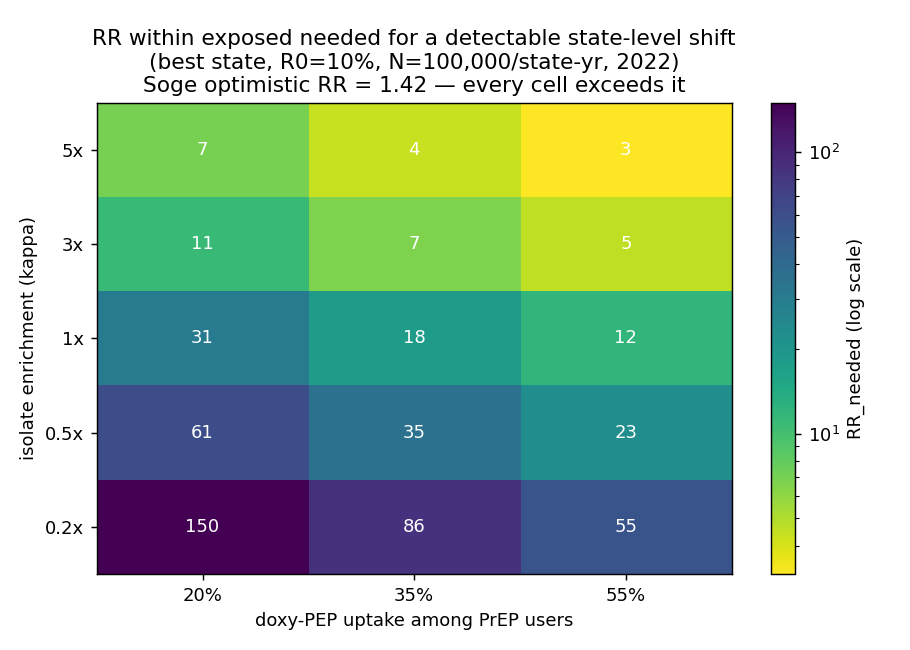
\includegraphics[width=0.82\textwidth,keepaspectratio]{feasibility_dilution.png}
\caption*{\textbf{Figure A. State level.} Within-exposed RR required for a
detectable state-level shift in tetracycline non-susceptibility, over doxy-PEP
uptake $\times$ isolate enrichment (combined PrEP+PLWH exposed, best state,
$R_0=10\%$, $N=100\,000$/state-year, 2024). Every cell exceeds the optimistic
benchmark RR~=~1.42 (minimum $\approx$1.9).}
\end{figure}
\noindent Alt text: A heatmap grid of doxy-PEP uptake against isolate enrichment
in which every cell shows a required relative risk above 1.42.

\begin{figure}[h]
\centering
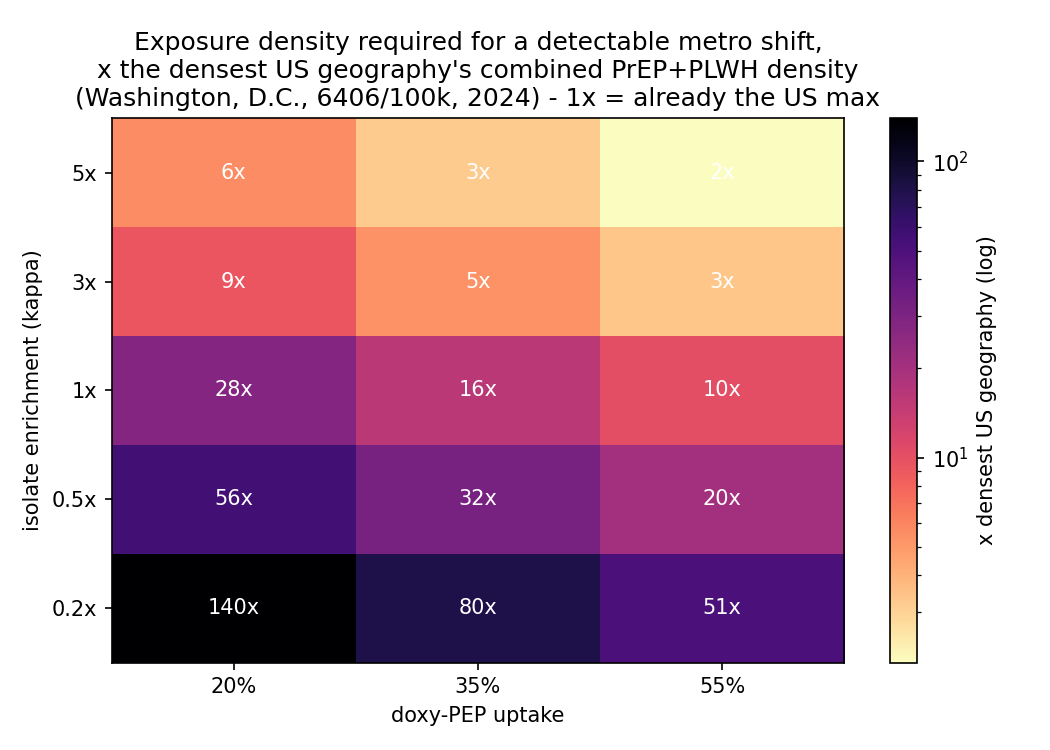
\includegraphics[width=0.82\textwidth,keepaspectratio]{feasibility_metro.png}
\caption*{\textbf{Figure B. Metro level.} Exposure density required for a
detectable shift, as multiples of the densest US geography's combined PrEP+PLWH
density (Washington, D.C., 6\,406/100\,000 adult males, 2024). $1\times$ is
already the national maximum; the best cell needs $\approx$2$\times$ it.}
\end{figure}
\noindent Alt text: A chart showing required combined PrEP+PLWH exposure density in
multiples of the densest US metropolitan geography, with all requirements above the
one-times national maximum.

\begin{figure}[h]
\centering

\includegraphics[width=0.82\textwidth,keepaspectratio]{feasibility_metro_breakeven.png}
\caption*{\textbf{Figure C. Break-even in proxy-free units.} Share of \emph{all}
adult males under combined PrEP+PLWH exposure required for detection versus
isolates per geography-year, by enrichment $\kappa$. Every curve sits above
D.C.'s observed combined density (6.4\%) and, under realistic isolate volumes,
above the 100\%-of-males physical ceiling.}
\end{figure}
\noindent Alt text: Break-even curves of the share of all adult males under
combined PrEP+PLWH exposure required for detection against isolate volume, all
lying above both the observed combined density (6.4\%) and the 100\% physical
ceiling.

% ===================================================================
\section*{S5. Literature attention structure}

A defined PubMed search (2015--2026; queries and a frozen result snapshot in the
repository) identified 361 doxy-PEP papers, of which 13 (3.6\%) mention a
bystander staphylococcal organism and only 2 measure tetracycline-resistant \sa{}
against a doxy-PEP exposure contrast. This is consistent with a research system
whose attention remains concentrated where its existing instruments already point,
and is not evidence of neglect by any author.

% ===================================================================
\section*{S6. Distributive observability}

The three streams share a measurement asymmetry that is a property of the
evidence architecture before it is a moral claim. The intervention's benefit and
the trial's resistance signal are identifiable within an exposed population:
exposure ascertained, denominator defined, phenotype measured, a longitudinal
causal contrast available. The population that would inherit a downstream
resistance consequence has none of these jointly --- no assigned measurement
mandate (Stream B) and no deployed system in which doxy-PEP exposure and the
\sa{} tetracycline phenotype share a denominator (Stream C). We call this
difference in scientific visibility \emph{distributive observability}: which
population remains represented by the evidence system, and at what inferential
resolution, once the question moves downstream from the treated to the affected
population. It does not establish that a population harm has occurred; it
establishes that, were one occurring, the deployed architecture could estimate the
intervention side of the benefit--externality ledger far more completely than the
externality side. An externality no instrument can price is not thereby small ---
it is unweighable, and an architecture that prices only one side of the ledger
cannot show that benefit outweighs external cost. The construct is built from
familiar parts (estimand mismatch; ascertainment and surveillance bias;
metric substitution of the Goodhart type) but concerns their coupling across an
evidence-production chain, and generalises to any intervention whose benefits
concentrate in an observed recipient population while its consequences diffuse
beyond it.

% ===================================================================
\section*{S7. Reproducibility}

All analysis is Python 3.11 (pandas, statsmodels, scipy, matplotlib); no
proprietary dependencies. Raw data are immutable; all cleaning is in code; every
figure and table regenerates from \texttt{make all}. Analysis decisions that could
go either way were logged with dates in \texttt{DECISIONS.md} before results were
known. All source files are SHA-256-pinned (\texttt{data/raw/**/CHECKSUMS.md}).
The repository is public and archived with a citable DOI.

\end{document}
